\documentclass[a4paper, 12pt]{article}
\usepackage[utf8]{inputenc}
\usepackage[T1]{fontenc}
\usepackage[french]{babel}
\usepackage{graphicx}
\usepackage{amsmath}
\usepackage{hyperref}
\usepackage{lmodern}
\usepackage{moreverb}
\usepackage{multicol}

\hypersetup{
    colorlinks=true,
    linkcolor=blue,
    filecolor=magenta,      
    urlcolor=cyan,
    pdftitle={Overleaf Example},
    pdfpagemode=FullScreen,
    }

\urlstyle{same}
\usepackage[a4paper,left=2cm,right=2cm,top=2cm,bottom=2cm]{geometry}

\pagestyle{headings}
\pagestyle{plain}


\setcounter{secnumdepth}{4}
\setcounter{tocdepth}{4}
\makeatletter


\makeatother



\makeatletter
\def\toclevel@subsubsubsection{4}
\def\toclevel@paragraph{5}
\def\toclevel@subparagraph{6}
\makeatother





\setlength{\parindent}{0cm}
\setlength{\parskip}{1ex plus 0.5ex minus 0.2ex}
\newcommand{\hsp}{\hspace{20pt}}
\newcommand{\HRule}{\rule{\linewidth}{0.5mm}}

\begin{document}

\begin{titlepage}
  \begin{sffamily}
  \begin{center}

   
    \textsc{\LARGE }\\[2cm]

    \textsc{\Large Compte rendu de Réunion}\\[1.5cm]
    \textsc{\Medium Rédigé par Mohammed ROUABAH }

    % Title
    \HRule \\[0.4cm]
    { \huge  \textsc{StellaStone} \\
    \textsc{\Large By Novus}\\ [0.4cm] }
	

    \HRule \\[2cm]
    \textsc {Idriss BENGUEZZOU\\Mohammed ROUABAH\\Ghilas MEZIANE \\ Ilyes ZEGHDALLOU}
 \begin{figure}
     \centering
    
\includegraphics[scale=0.2]{logoUJM.png}
     \label{fig:ujm_logo}
 \end{figure}
   
    \

    \vfill

    % Bottom of the page
    {\large {} 28/10/2022}

  \end{center}
  \end{sffamily}
\end{titlepage}

\newpage

\section{Réunion du Vendredi 28/10}
La réunion de cette semaine s'est déroulée le vendredi 28 octobre 2022 en distanciel, sur notre propre serveur discord sur le créneau horaire 18h-19h, avec la présence de tous les membres : Idriss BENGUEZZOU-Mohammed ROUABAH-Ghilas MEZIANE- Ilyes ZEGHDALLOU. \\

\textbf{Ordre du jour :}
 \begin{itemize}
     \item Relecture des nouvelles exigences rédigées par chacun. 
     \item Observation de l'avancement du document tests de recette.
 \end{itemize}


\section{Un tour de table}

Chaque membre a exposé les exigences écrites pendant la semaine au reste du groupe. \\

En premier, Mr.ZEGHDALLOU Ilyes, a terminé la rédaction des exigences concernant la
page d’authentification,la sécurité, ainsi que les exigences concernant l'édition du profil utilisateur. Par conséquent, son issue TRELLO a été clôturée. \\

Mr.MEZIANE Ghilas a présenté son avancement sur la partie construction de la fusée. Il nous a également présenté l'interface d'un ancien jeu nommé Robocraft qui pourrait nous servir de modèle. \\ 

Voici la vidéo présentée : 
\href{https://www.youtube.com/watch?v=dA4f3Skk01o&ab_channel=Robocraft2}{vidéo du jeu Robocraft}
\\ \\
Mr.BENGUEZZOU Idriss, a présenté les exigences qu'il a rédigé concernant le réseau social intégré à notre application nommé 'Réseau spatial'.
\\

Mr.ROUABAH a quant à lui avancé sur les exigences de la partie Entreprise et les rapports de simulation.

Aussi, nous avons effectué à tour de rôle une relecture du document de test des recettes suite à notre réunion exceptionnelle datant du 25/10/2022 qui avait pour but,justement, d'avancer sur ce document.
\newpage
\section{Une mise à niveau}

Nous avons également durant cette réunion décidé de reprendre ensemble les principales interfaces que nous avions imaginé et de les représenter sous forme de schéma pour avoir une vision globale du projet.
\\
 \begin{figure}[!h]
    \centering
    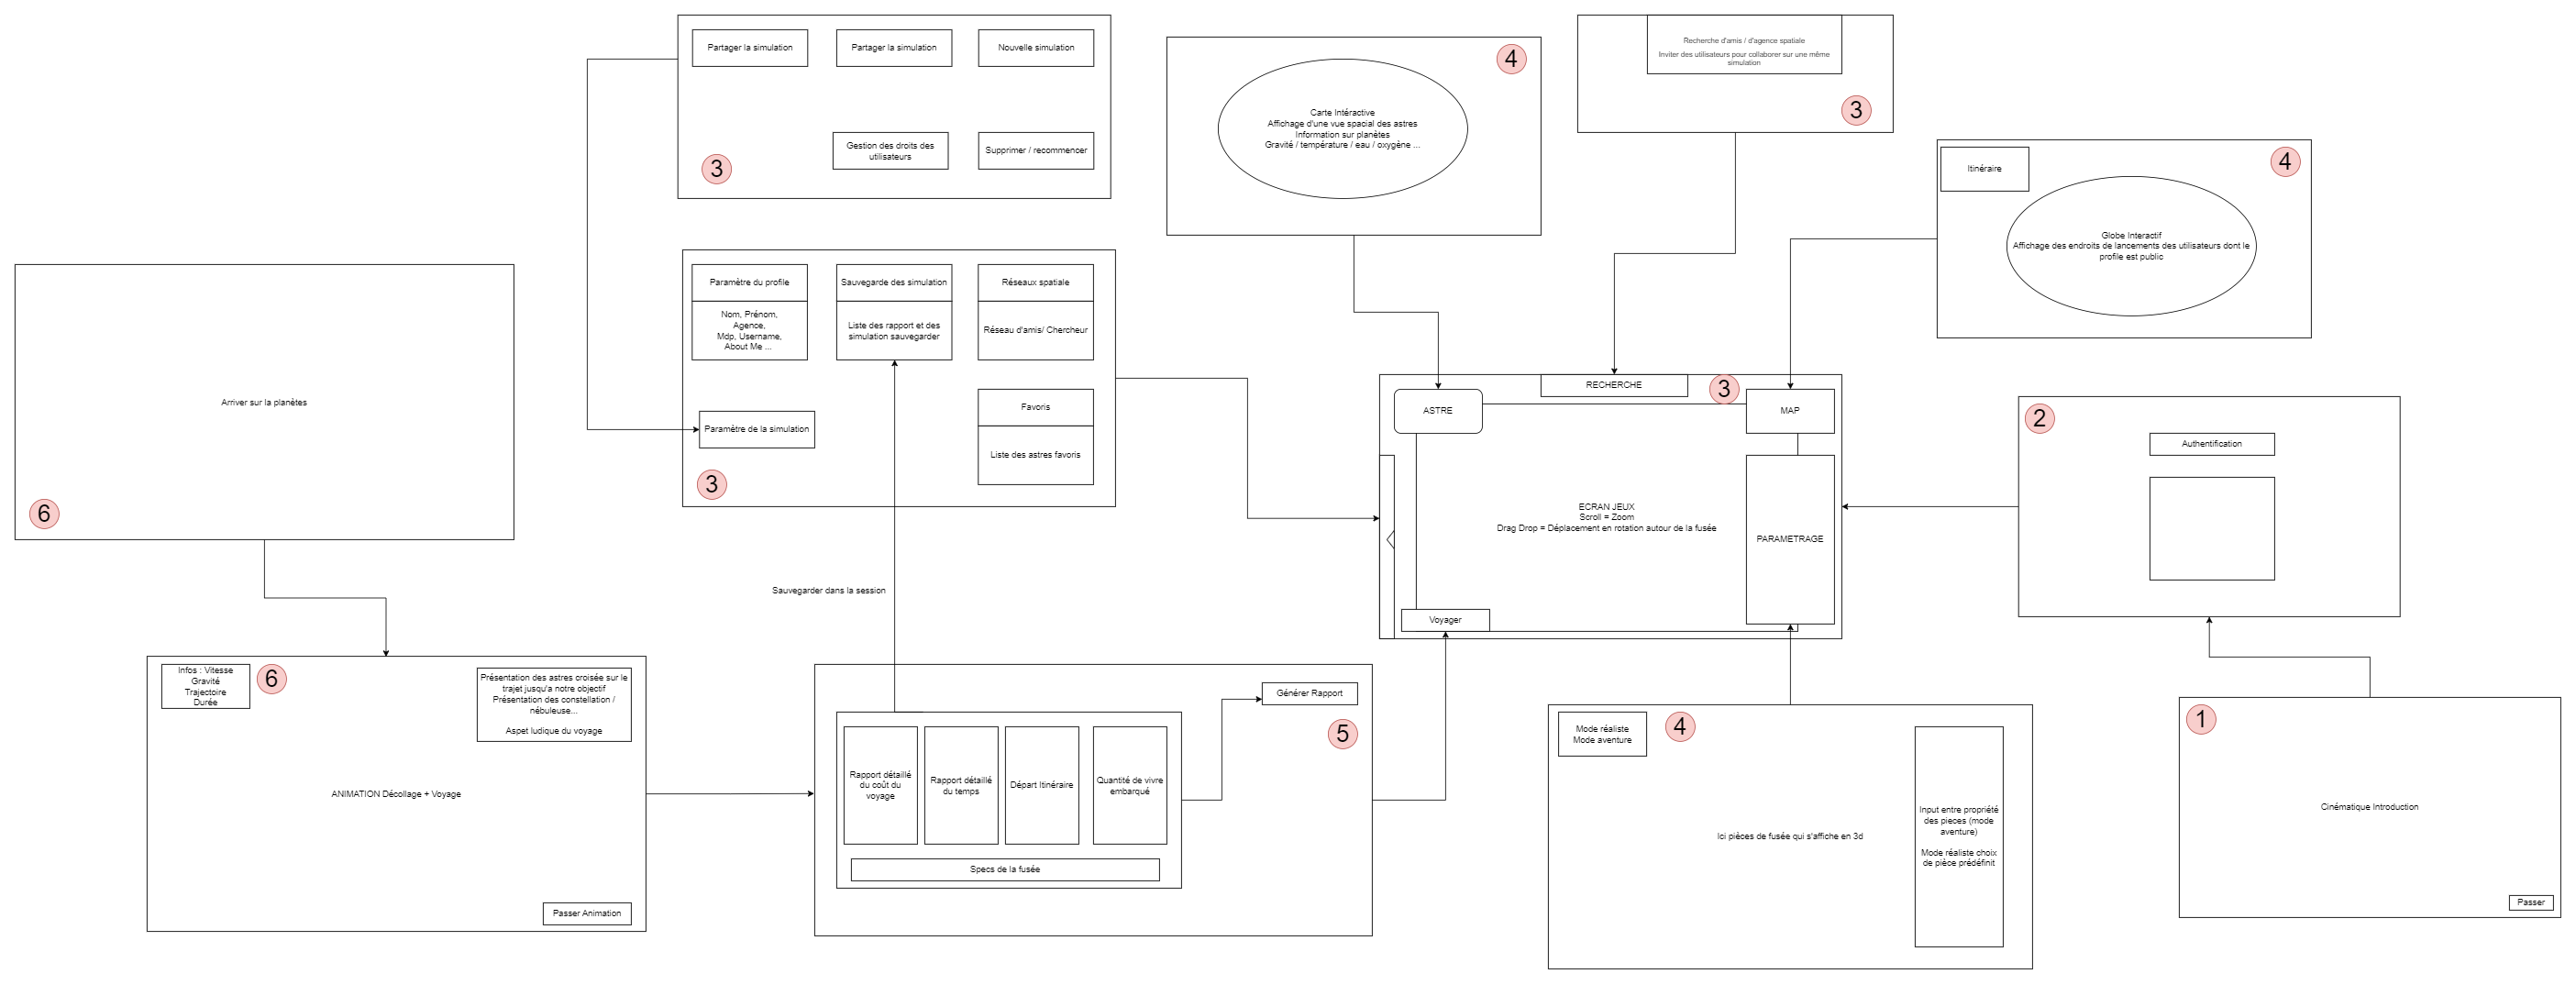
\includegraphics[scale=0.18]{overview.png}
    \label{fig:Le_planning}
    \caption{Overview}
\end{figure}



\section{Prochaine réunion et objectifs de la semaine}
En raison du partiel d'intelligence artificielle, nous avons décidé de ne pas nous réunir le vendredi prochain. Par conséquent,la prochaine réunion est fixée pour le vendredi 11 novembre 2022, sur le créneau horaire 17h-18h avec pour ordre du jour:
\\

\begin{itemize}
    \item Révision du document de spécification des exigences,
    \item Révision du document de tests de recette,
    \item Introduction au document de conception générale. \\
\end{itemize}

La prochaine personne en charge de la rédaction du compte rendu de réunion est : ZEGHDALLOU Ilyes.

\end{document}